\documentclass{standalone}
\usepackage{testpiece}

\begin{document}
\begin{tikzpicture}
\node[anchor=north west, rotate=20, transform shape, inner sep=0pt] (cornet) at (0,-1.3cm) {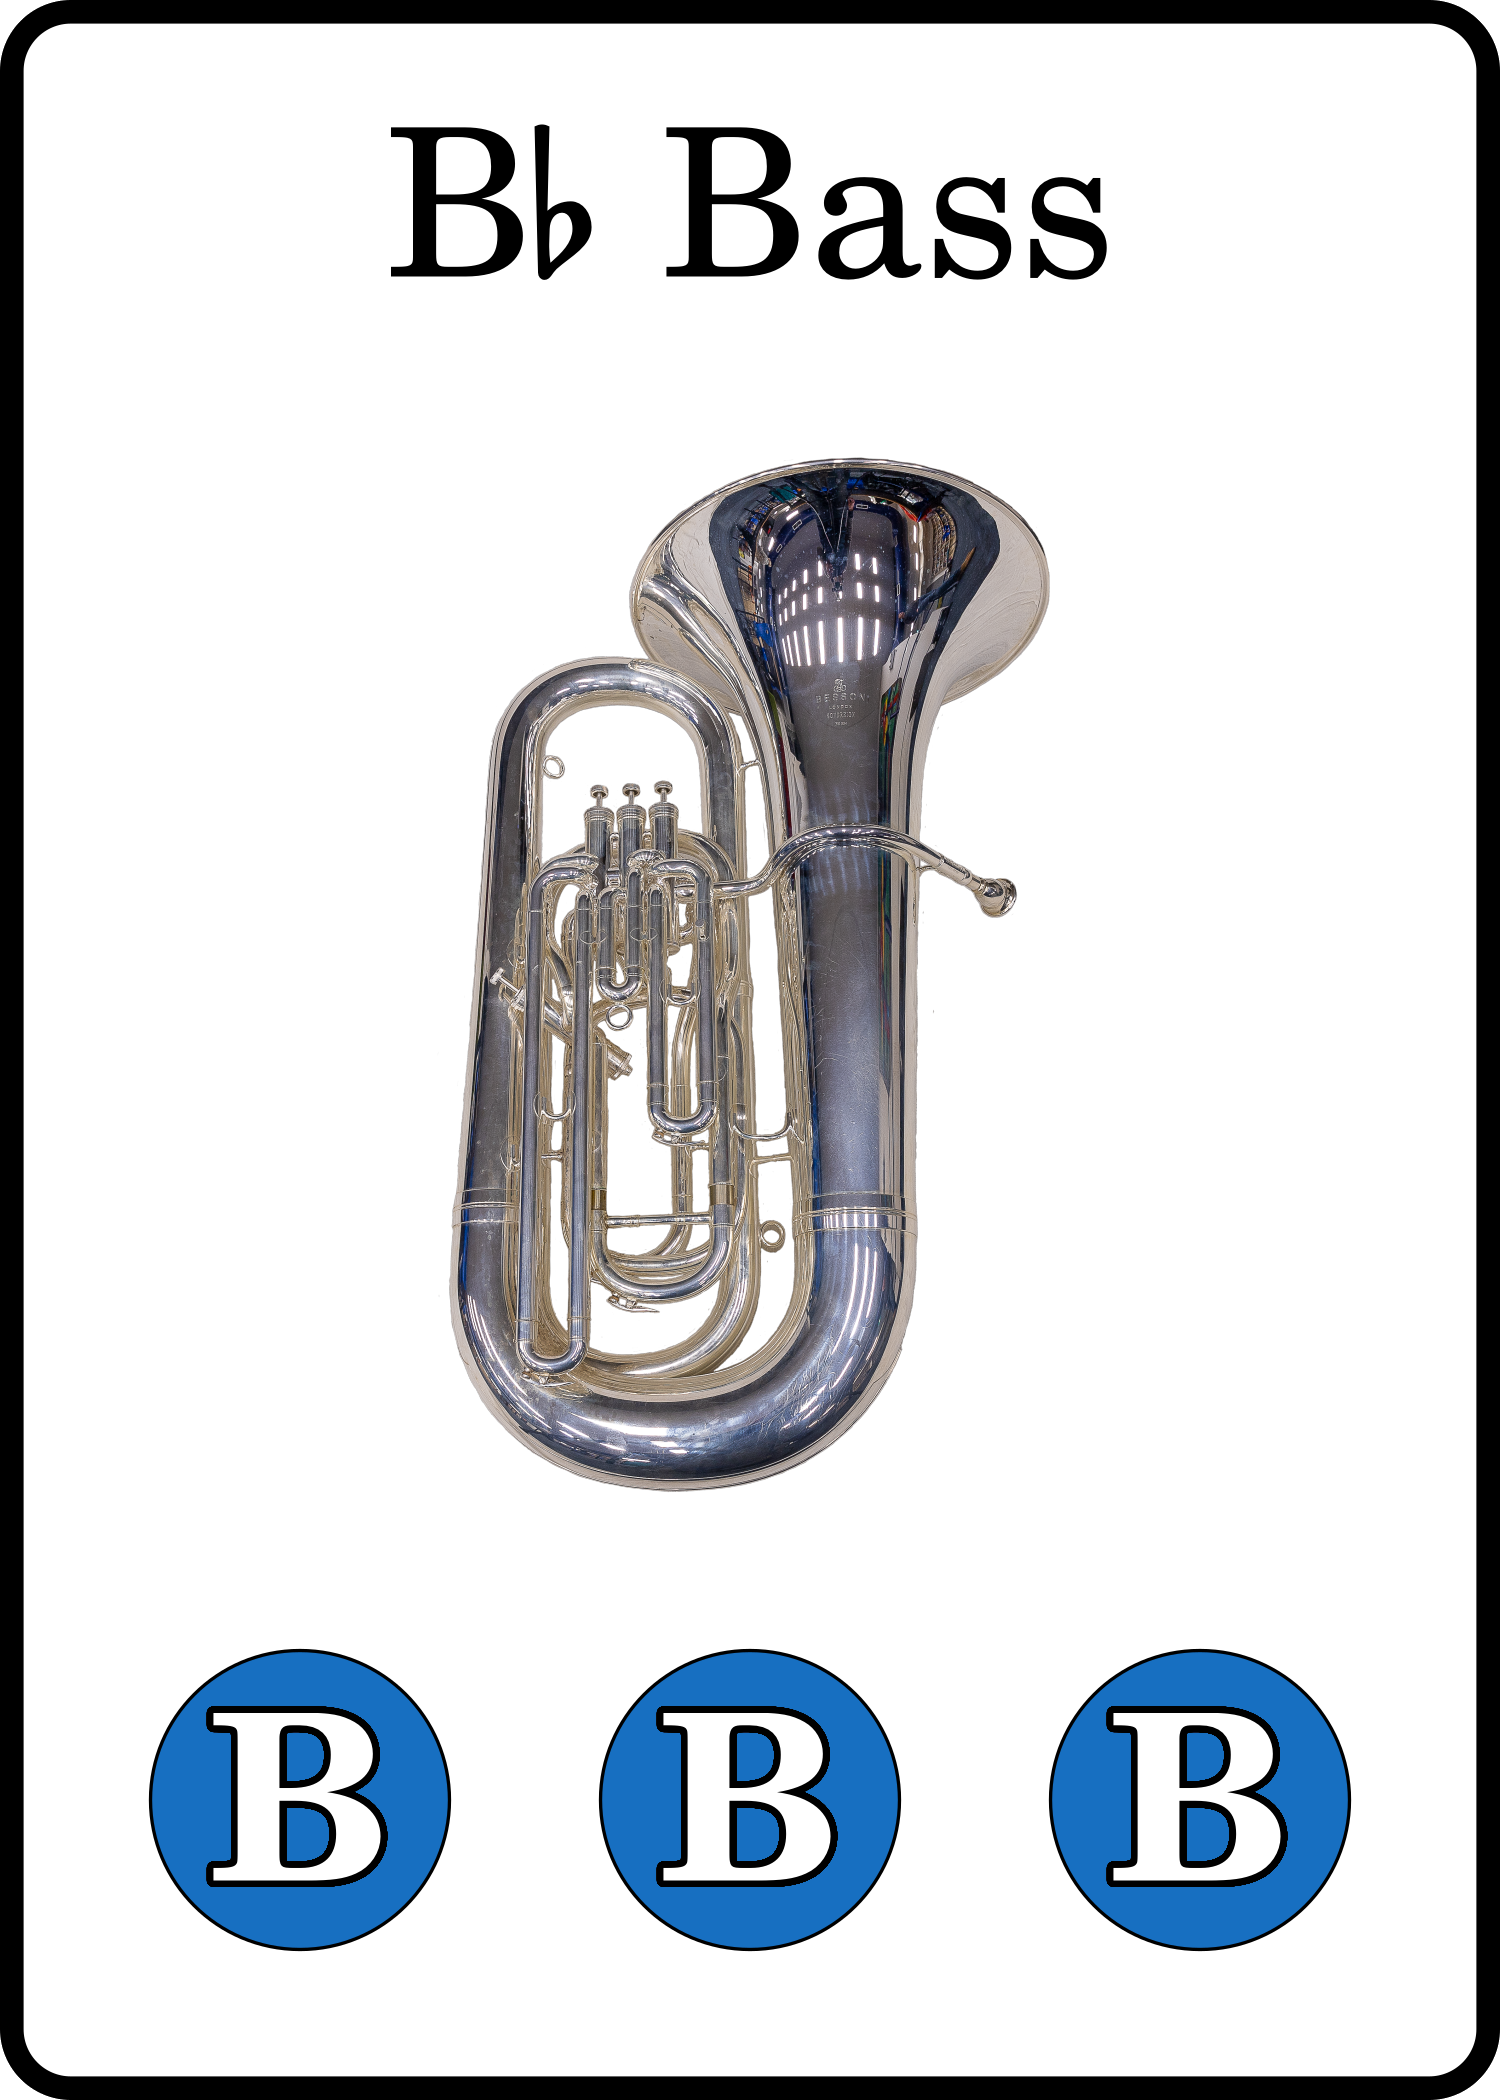
\includegraphics[height=3.75cm]{Images/CardImages/bass_display_front.png}};
\node[anchor=north, rotate=0, transform shape, inner sep=0pt] at (36mm, -0.45cm) (cornet) {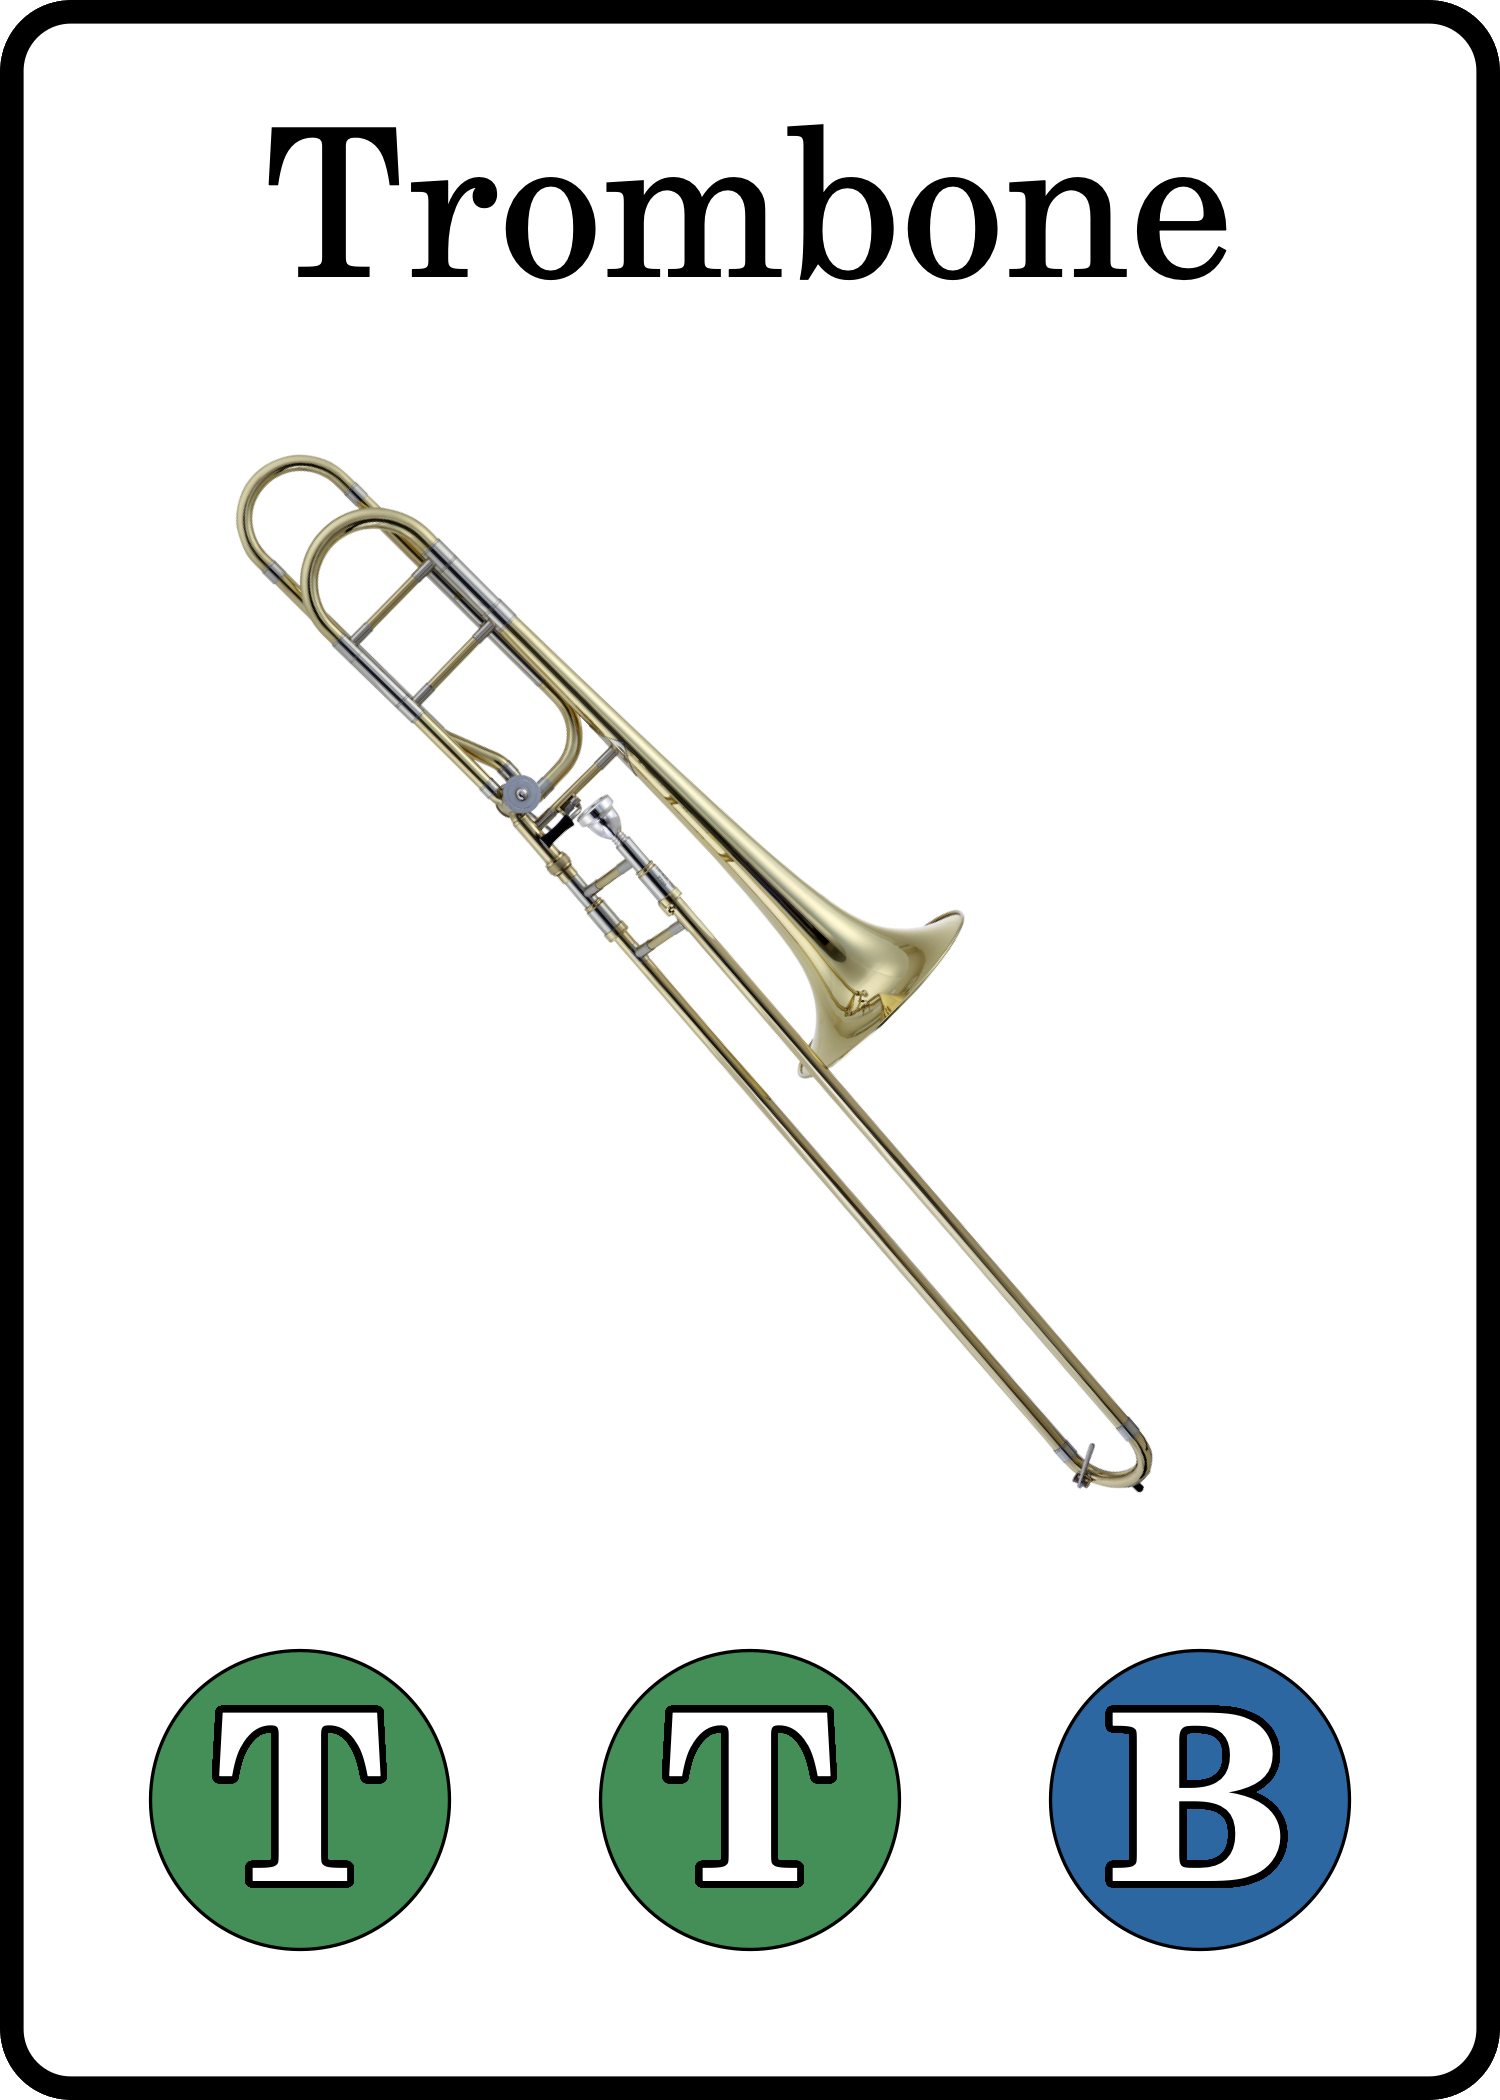
\includegraphics[height=3.75cm]{Images/CardImages/trombone_display_front.png}};
\node[anchor=north east, rotate=-20, transform shape, inner sep=0pt] at (72mm, -1.3cm) {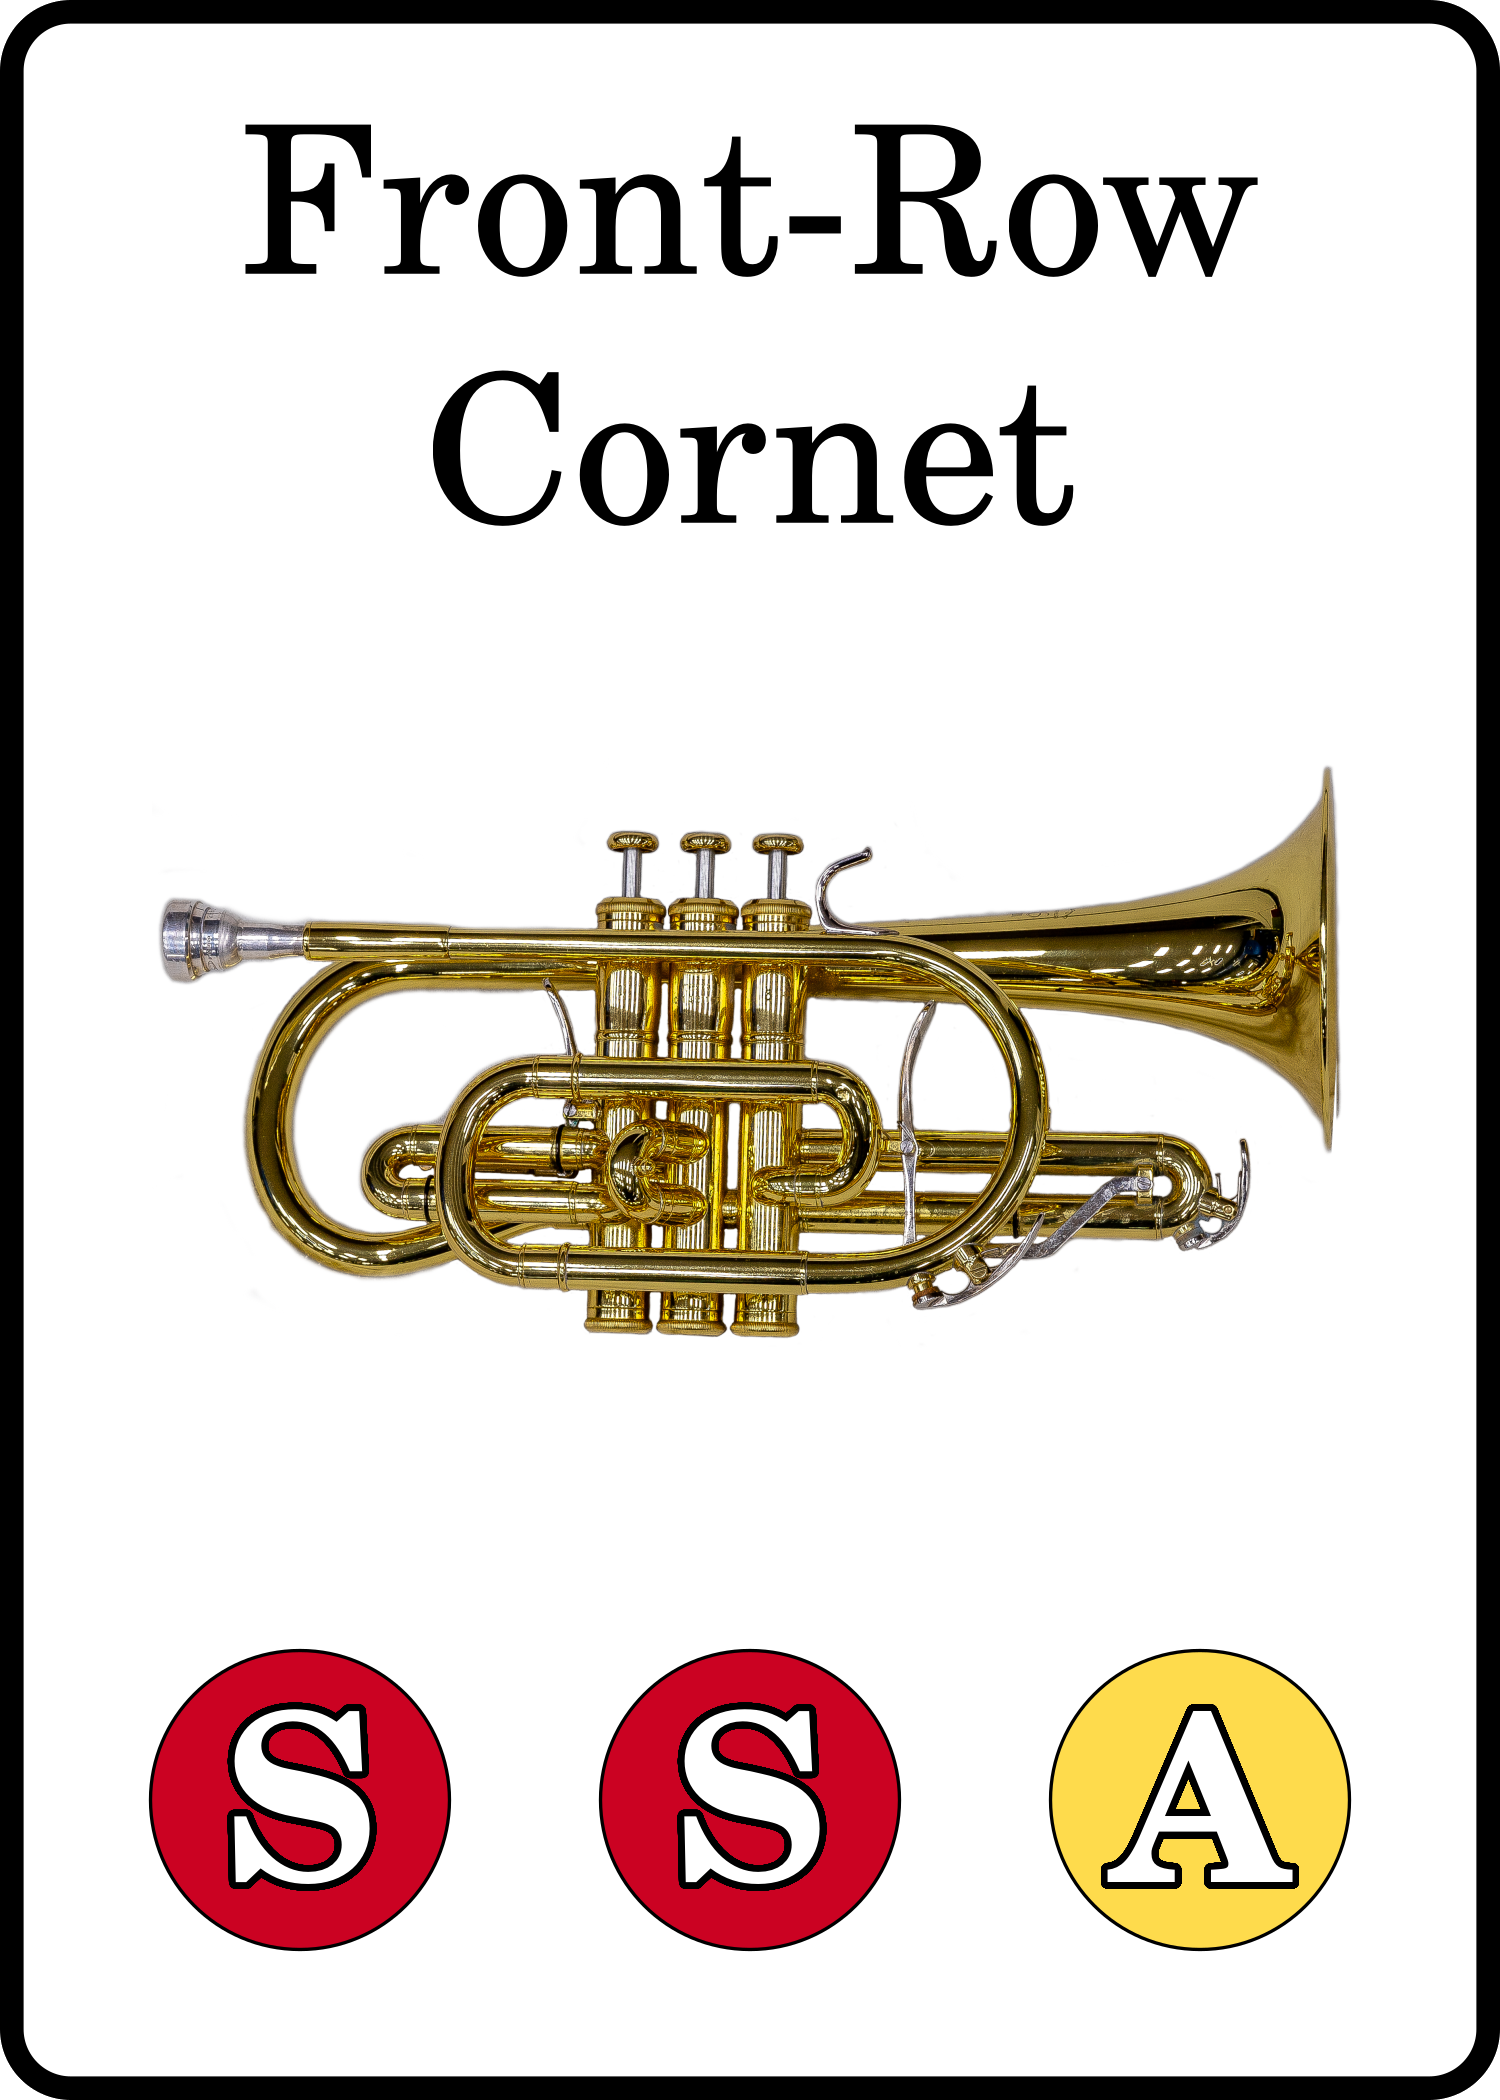
\includegraphics[height=3.75cm]{Images/CardImages/cornet_display_front.png}};
\end{tikzpicture}
\end{document}